\section{Prototipo realizacija}

Šis skyrius aprašo praktinę rašto darbo pusę -- debesų kompiuterijos technologijomis grįstos saityno peržvalgos roboto sistemos implementaciją ir jos niuansus. Architektūra ir naudojami įrankiai parinkti pagal 4 skyriuje apibrėžtus sistemos reikalavimus.

\subsection{Naudojama architektūra}

Prototipas rengiamas plačiai remiantis Kalifornijos Mersedo universiteto mokslininkų literatūrine medžiaga apie debesų kompiuterijos išskirstyto saityno žvalgymo roboto sistemą ir jos architektūrą, dizaino principus \cite{MercedCloudBasedWebCrawler}. Atsižvelgiant į darbo rašymo metus ir patobulėjusias debesų kompiuterijos tiekėjų siūlomas technologijas, pasiūlyta architektūra realizuojama pritaikius specifinius pokyčius pakeičiant realizacijos įrankius ar platformas.  

\begin{figure}[ht]
\centering
\includegraphics[scale=0.6]{img/Mersed_architektūra.png}
\caption{Mersedo universiteto mokslininkų pasiūlyta saityno peržiūros roboto architektūra \cite{MercedCloudBasedWebCrawler}}
\label{fig:mersed_architecture}
\end{figure}

\subsubsection{Centrinis žvalgymo variklis}
 
 Tai pagrindinis sistemos struktūrinis komponentas, kuris inicijuoja visą žvalgymo procesą ir kuria/naikina žvalgymo agentus. Pagrindiniai šio komponento veikimo etapai:
 \begin{enumerate}
     \item Inicializacija
     \begin{enumerate}
         \item Paimami pradiniai URL adresai iš žvalgymo adresų sąrašo
         \item Adresai sudedami į „Azure“ eilę prieš tai patikrinant, ar kiekvienas URL dar nebuvo žvalgytas („Azure NoSQL Table Storage“)
         \item Sukuriamas pirmasis žvalgymo agentas, jam priskiriama jo žvalgymo zona (svetainės serverio vardas)
     \end{enumerate}
     \item Ciklinis žvalgymo procesas
     \begin{enumerate}
         \item Iš žvalgymo eilės paimamas URL adresas
         \item Patikrinama, ar esama adresui egzistuoja aktyvus agentas (SQL Agentų registro duombazė)
         \item Jei agentas egzistuoja, URL ignoruojamas, nes agentas jį apdoros
         \item Jei aktyvaus agento nėra, tikrinamas maksimalus leistinas agentų skaičius, jei jis neviršytas, bandoma sukurti naują agentą ir jam priskirti URL adreso vardo zoną.
         \item Kartojama nuo pirmo žingsnio
     \end{enumerate}
 \end{enumerate}
 
 \subsubsection{Žvalgymo agentas}

Šis komponentas iš žvalgymo eilės ima URL adresą, jei adreso vardo sritis sutampa su agentui priskirtu aptarnavimo vardo adresu, jis inicijuoja HTTP užklausą į nurodytą žiniatinklio serverį, parsiunčia HTML turinį, išgauna visas jame esančias nuorodas, kiekvienai jų patikrina, ar nuoroda dar neregistruota indeksų repozitorijoje ir atitinkamai perduoda aktyviam žvalgymo agentui, kurio zona sutampa su URL adreso vardo zona. Agentai užtikrina išskirstytos sistemos veikimo principą, juos dinamiškai galima pridėti, šalinti.

 \subsubsection{Agentų registras}
 
 Tai SQL duombazė, kurioje registruojami visi aktyvūs agentai, taip pat išregistruojami. Šis komponentas yra bendras, todėl rašto darbo paskutiniame skyriuje, atliekant tyrimą, bus analizuojama, ar jis negali lemti „butelio kaklelio“ efekto.
 
 % Table generated by Excel2LaTeX from sheet 'crawling_vs_scraping'
\begin{table}[htbp]
  \centering
  \caption{Agentų registro lentelės schema \cite{MercedCloudBasedWebCrawler}}
    \begin{tabular}{|l|l|l|l|l|}
    \hline
    \textbf{Id} & \textbf{Agento\_Vardas} & \textbf{Agento\_Aptarnavimo\_Sritis} & \textbf{\textcolor{red}{Paskutinis\_Aktyvumas}} & \textbf{Ištrintas} \bigstrut\\
    \hline
    1 & A1 & abc.lt & 2020-05-02 15:30:15 & false \\
    \hline
    2 & A2 & def.lt & 2020-05-02 13:30:15 & true \\
    \hline
    \end{tabular}%
  \label{tab:agent_registry_table}%
\end{table}%
 
 \ref{tab:agent_registry_table} lentelėje pavaizduotoje agentų registro lentelėje raudonai pažymėtas paskutinio aktyvumo laiko stulpelis originaliai \cite{MercedCloudBasedWebCrawler} literatūroje neminėtas, tai -- rašto darbo autoriaus prototipo planavimo metu įgyvendinta korekcija siekiant atlaisvinti nebenaudojamus agentus.
 
 \subsubsection{„Azure“ žvalgymo eilė}
 
 Tai komponentas, kuris saityno žvalgymo sistemų literatūroje minimas kaip „žvalgymo pasienio“ (angl. -- \textit{Crawling Frontier}) komponentas, kuriame laikinai kaupiami žvalgytinų puslapių URL adresai. Žvalgymo agentai ir Centrinis žvalgymo variklis klausosi šios eilės žinučių ir jas apdoroja. Tai dar vienas bendrinis sistemos komponentas, todėl eksperimento metu taip pat bus stebimas jo veikimo pralaidumas. \cite{MercedCloudBasedWebCrawler} moksliame darbe jau buvo atliktas šio komponento tyrimas ir įsitikinta, kad didinant žinučių kiekio apkrovą, komponento pralaidumas išlieka gana patovus. Naudota „Azure Storage Queues“ eilių paslauga. Šio rašto darbo tyrime bus naudojama kita „Azure“ paslaugų eilių infrastruktūra, todėl taip pat pakartotinai bus stebimas komponento veikimo optimalumas.
 
 \subsubsection{„Azure“ NoSQL indeksų repozitorija}

Tai NoSQL rakto-reikšmės (angl. -- \textit{Key-Value}) tipo saugykla, kurioje agentai registruoja identifikuotus svetainių URL adresus, taip pat keičia tų adresų žvalgymo statusą.

\subsubsection{„Azure“ didelių objektų saugykla}

Šis komponentas aprašytoje architektūroje atsakingas už didelių multimedijos failų saugojimą -- nuotraukų, vaizdo įrašų, dokumentų, kitų žiniatinklio resursų, kurie nėra HTML dokumentai. Pasižymi tuo, jog gali talpinti didelius kiekius duomenų.

\subsubsection{Svetainės turinio analizatorius ir dublikatų aptikimas}

Vienas iš minimų sistemos komponentų -- svetainės turinio analizatorius -- semantiškai apdoroja nuskaitytą HTML dokumento turinį siekdamas nustatyti puslapio tematiką, pagrindinius raktinius žodžius, taip pat identifikuoti pasikartojančio, dublikuoto turinio svetaines. Šio prototipo įgyvendinimo ribose nebuvo numatytas semantinis svetainės turinio analizavimas, todėl plačiau šie komponentai aptariami nebus.

\subsubsection{Decentralizuota komunikacija}

Aprašomos saityno peržvalgos roboto sistemos architektūros išskirtinis bruožas lyginant ją su anksčiau nagrinėtomis literatūroje aprašytomis sistemomis -- nepriklausomas agentų veikimas ir apsikeitimas žvalgytinais puslapiais be centrinio darbo koordinavimo komponento \cite{MercedCloudBasedWebCrawler} (centrinis žvalgymo variklis nekoordinuoja darbo, tik valdo agentų gyvavimo ciklą). Šis išskirtinumas leidžia plėsti sistemos žvalgymo pajėgumus pridedant naujus žvalgymo agentus, kurie savo žvalgymo rezultatus gali perduoti kitiems agentams tiesiogiai be tarpinio komponento. Kiekvienas agentas turi priskirtą aiškia žvalgymo zoną (domeną), todėl atlieka tik savo srities žvalgymo atominę operaciją.

\subsection{Struktūrinis prototipo dizainas}

Šiame poskyryje aprašoma koreguota \cite{MercedCloudBasedWebCrawler} mokslininkų pasiūlyta išskirstyto saityno peržvalgos roboto sistemos struktūrinė architektūra. Ji detalizuojama aprašant naudojamas „Microsoft Azure“ debesų kompiuterijos infrastruktūros tiekėjo paslaugas ir resursus. Rašto darbe įgyvendinant prototipą pasirinktas pastarasis debesų kompiuterijos sprendimas dėl rašto darbo autoriaus patirties naudojantis jo paslaugomis, tačiau nėra problemų šią architektūrą realizuoti su bet kuriuo kitu debesų kompiuterijos paslaugų tiekėju (pvz.: Amazon Web Services arba Google Cloud Platform).

\pagebreak

Paeiktoje \ref{fig:azure_implementation_structural_scheme} schemoje detalizuojami esminiai sistemos struktūriniai komponentai ir jų „Azure“ platformos infrastruktūros paslaugų rūšys. 
\begin{figure}[htp!]
\centering
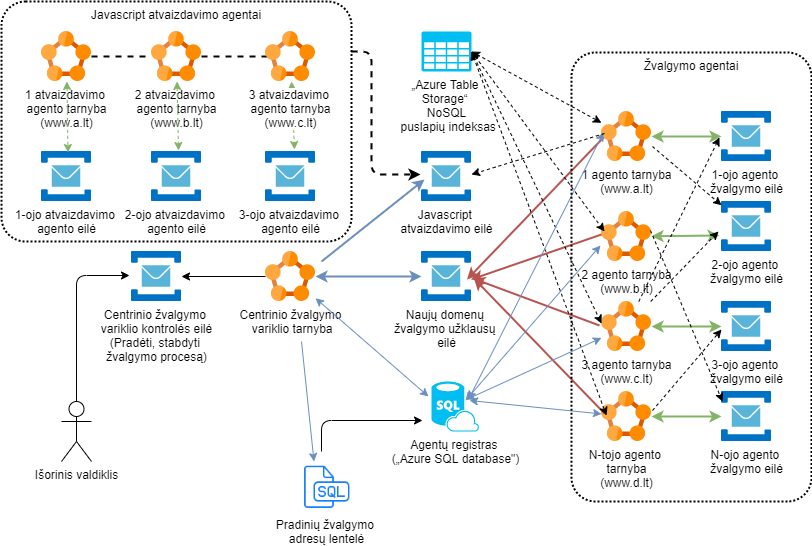
\includegraphics[scale=0.6]{img/Azure_Implementacija_Kasparo.png}
\caption{Struktūrinė prototipo sistemos schema}
\label{fig:azure_implementation_structural_scheme}
\end{figure}

\subsubsection{Sistemos orchestravimo platforma}

Įgyvendinant detalųjį architektūrinį saityno peržvalgos roboto sistemos dizainą ir renkantis iš technologijų, buvo pasirinkta „Microsoft Azure Service Fabric“ mikroservisų orchestravimo platforma, kuri apibrėžia ne tik sistemų klasterių valdymą ir išplėtimą, tačiau taip pat turi savo vykdomąją aplinką (angl. -- \textit{Service Fabric Runtime Environment}), kuri palaiko „Service Fabric“ programavimo modelius. Alternatyvi galimybė buvo rinktis „Azure Kubernetes Service“ orchestratoriaus paslaugą, tačiau „Service Fabric“ buvo pasirinktas dėl didelių vykdomosios aplinkos ir programavimo modelių galimybių, kurios suteikia daug abstrakcijos programuotojams -- leidžia orientuotis į verslo kodo rašymą paliekant infrastruktūrines surišimo problemas pačiai platformai.

\subsubsection{„Service Fabric“ infrastruktūra}

Šios platformos infrastruktūros konceptą apibrėžia 3 pagrindiniai komponentai \cite{ServiceFabricTerminology}:
\begin{itemize}
    \item Klasteris (angl. -- \textit{Cluster}) -- tinklu sujungtas išplečiamas rinkinys virtualių ar fizinių mašinų, kuriose diegiami „Service Fabric“ programų paketai, gali turėti kelis priskirtus mazgo tipus
    \item Mazgo tipas (angl. -- \textit{Node Type}) -- komponentas, kuris sujungia „Service Fabric“ klasterį su „Azure“ virtualių mašinų rinkiniu. Gali turėti ne daugiau nei vieną priskirtą virtualių mašinų rinkinį
    \item Virtualių mašinų išplėtimo rinkinys (angl. -- \textit{Virtual Machine Scale Set}) -- virtualių mašinų kolekciją, kurioje galima pridėti/trinti mašinas
    \item Mazgas (angl. -- \textit{Node}) -- virtuali arba fizinė mašina, kuri yra sudedamoji klasterio dalis, turi priskiriamą vardą
\end{itemize}

\begin{figure}[htp!]
\centering
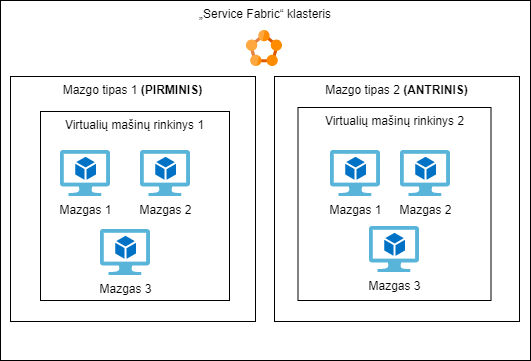
\includegraphics[scale=0.7]{img/SF_infrastructure.png}
\caption{„Service Fabric“ infrastruktūra \cite{ServiceFabricTerminology}}
\label{fig:sf_infrastructure}
\end{figure}

\ref{fig:sf_infrastructure} matomas infrastruktūros komponentų išsidėstymas. Vienas mazgo tipas visada būna pirminis, o kiti -- antriniai. Pirminio mazgo tipo virtualių mašinų korekciją nerekomenduojama, nes gali turėti tiesioginės įtakos klasterio veikimui.

\subsubsection{„Service Fabric“ programavimo modelis}

„Service Fabric“ programavimo modelį sudaro šie pagrindiniai komponentai:

\begin{itemize}
    \item Programa (angl. -- \textit{Application})
    \item Tarnyba (angl. -- \textit{Service})
    \item Skaidinys (angl. -- \textit{Partition})
    \item Kopija (angl. -- \textit{Replica})
\end{itemize}

\begin{figure}[htp!]
\centering
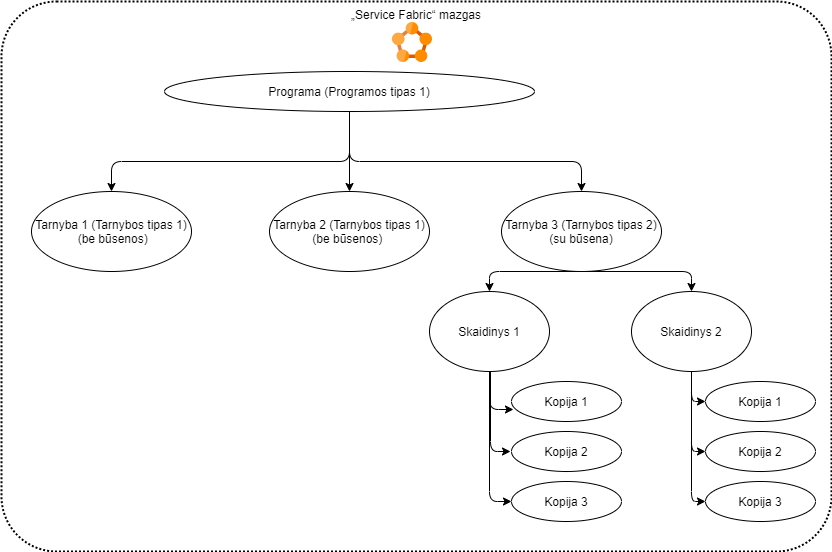
\includegraphics[scale=0.5]{img/SF_programming_model.png}
\caption{„Service Fabric“ programavimo modelis \cite{ServiceFabricTerminology}}
\label{fig:sf_programming_model}
\end{figure}

\subsubsection{Žvalgymo agentai}

//TODO aprašyti žvalgymo agentus kaip Service Fabric Stateless Services, paaiškinti, kaip jie komunikuoja su atitinkamomis eilėmis

\subsubsubsection{„Azure Service Bus“ eilės}

//TODO aprašyti žvalgymo, centrinio žvalgymo tarnybos, atvaizdavimo eiles, taip pat naujų domenų žvalgymo užklausų eilę.

\subsubsection{„Azure Table Storage“ indekso saugyklos struktūra}


\subsubsection{Dinaminė sistemos veikimo schema}

// TODO: UML Sequence diagrama.

\subsubsection{Kiti prototipo realizacijoje panaudoti įrankiai}

// TODO: .NET Core 3.1, Dapper, C\# AbotCrawler biblioteka žiniatinklio žvalgymui